\documentclass[
  accentcolor=tud1c,	% Color theme for TUD corporate design
  colorbacktitle,		% Titlepage has colored background for title area
  inverttitle,			% Font color of title on titlepage is inverted
  german,				% Document is in english
  twoside
]{tudexercise}

\usepackage[ngerman]{babel}
\usepackage{units}
\usepackage{hyperref}
\usepackage[utf8]{inputenc}
\usepackage{algorithm2e}

\definecolor{commentgreen}{RGB}{50,127,50}


\usepackage{listings}
\usepackage{listings}
\lstloadlanguages{C++}
\lstset{language=C++}
\lstset{captionpos=b}
\lstset{tabsize=3}
\lstset{breaklines=true}
\lstset{columns=flexible,keywordstyle=\color{purple},stringstyle=\color{blue},commentstyle=\color{commentgreen}}
\lstset{literate=%
{Ö}{{\"O}}1
{Ä}{{\"A}}1
{Ü}{{\"U}}1
{ß}{{\ss}}2
{ü}{{\"u}}1
{ä}{{\"a}}1
{ö}{{\"o}}1
{'}{{\textquotesingle}}1
}

\parindent0pt

\newcommand{\tag}{3}

\title{Übung zum\linebreak[1]C/C++-Praktikum\linebreak[1] Fachgebiet Echtzeitsysteme}
\subtitle{Übungen für den \tag{}. Tag}

\begin{document}

\begin{examheader}
	\textmb{Übung zum C/C++-Praktikum - Tag \tag{}}
\end{examheader}
\maketitle 

\vspace{5mm}

\section{Vererbung und Polymorphie}
\begin{enumerate}
\item Schreiben Sie eine Klasse \emph{Person}. \emph{Person} soll ein \emph{protected} Attribut \emph{name} vom Typ \emph{std::string} haben (\textbf{\#include <string>}), welches den Namen speichert. Initialisieren Sie den Namen im Konstruktor von \emph{Person} und schreiben Sie auch einen Destruktor. Implementieren Sie außerdem die Methode 
\begin{lstlisting}
std::string getInfo() const;
\end{lstlisting}

um Informationen über die Person, in unserem Fall den Namen, abzurufen. Hinweis: Um ein String-Literal an eine \emph{std::string} Variable anzuhängen, müssen Sie aus dem String-Literal zuerst ein \emph{std::string}-Objekt machen. Beispiel:
\begin{lstlisting}
std::string text = std::string("Name: " ) + name;
\end{lstlisting}

\item Schreiben Sie eine Klasse \emph{Student}, die von \emph{Person} erbt und eine Person mit einer Matrikelnummer (ebenfalls \emph{std::string}) modelliert. Rufen Sie in der Initialisierungsliste den entsprechenden Konstruktor der Elternklasse \emph{Person} mittels \textbf{Person(name)} auf. Implementieren Sie auch einen Destruktor. \\

Überschreiben Sie die Methode \emph{getInfo()}, sodass zusätzlich zum Namen auch die Matrikelnummer zurückgegeben wird. Sie können bei Bedarf die \emph{getInfo()}-Implementierung der Elternklasse \emph{Person} von \emph{Student} aus mittels \textbf{Person::getInfo()} aufrufen.

\item Erstellen Sie nun in der \emph{main()} eine je eine Person und einen Studenten und geben Sie deren Daten auf der Konsole aus. Vergewissern Sie sich, dass bei \emph{Student} auch die Matrikelnummer ausgegeben wird. Schauen Sie sich auch die Ausgaben der Konstruktoren und Destruktoren an, und versuchen Sie, diese nachzuvollziehen.

\item Implementieren Sie nun die Funktion 
\begin{lstlisting}
/** prints person information on console */
void printPersonInfo(const Person* p);
\end{lstlisting}

Dadurch, dass \emph{p} als const Zeiger übergeben wird, können auch Unterklassen von \emph{Person}, wie z.B. \emph{Student}, übergeben werden. \\

Testen Sie Ihre Implementierung. Rufen Sie dazu \emph{printPersonInfo()} sowohl mit beiden Personentypen auf.

\item Sie werden merken, dass \emph{printPersonInfo()} unabhängig von übergebenem Personentyp immer nur den Namen der Person ausgibt, aber nicht die Matrikelnummer. Der Grund dafür ist, dass \emph{getInfo()} nicht als \textbf{virtual} deklariert wurde und deshalb auch kein dynamischer Dispatch der Methode stattfindet. Deklarieren Sie daher \emph{getInfo()} als \textbf{virtual}. \\

Testen Sie Ihre Implementierung erneut und vergewissern Sie sich, dass nun immer die richtige Methode aufgerufen wird.

\item Legen Sie einen Studenten dynamisch auf dem Heap an, speichern Sie die Adresse jedoch in einem Zeiger auf eine \emph{Person}. Löschen Sie die Person anschließend.
\begin{lstlisting}
	Person* pTim = new Student("Tim", "321654");
	delete pTim;
\end{lstlisting}

Analysieren Sie die Konsolenausgabe. Wie Sie sehen, wird nur der Destruktor von \emph{Person} aufgerufen, obwohl es sich um ein Objekt vom Typ \emph{Student} handelt. Auch hier liegt es daran, dass kein dynamischer Dispatch bei der Zerstörung erfolgt. Deklarieren Sie deshalb in beiden Klassen den Destruktor als \textbf{virtual} und testen Sie die Korrektheit der Destruktoraufrufe.

\end{enumerate}


\section{Pure Virtual}
In dieser Aufgabe wollen wir Vererbung und Polymorphie dazu nutzen, um mathematische Ausdrücke als Bäume von Primitivoperationen zu modellieren. Dazu werden wir eine abstrakte Oberklasse \emph{Expression} mit der abstrakten Methode \emph{compute()} erstellen. Einzelne Knotentypen wie Addition und Subtraktion werden von \emph{Expression} abgeleitet und implementieren \emph{compute()}, um die jeweilige Operation zu realisieren.

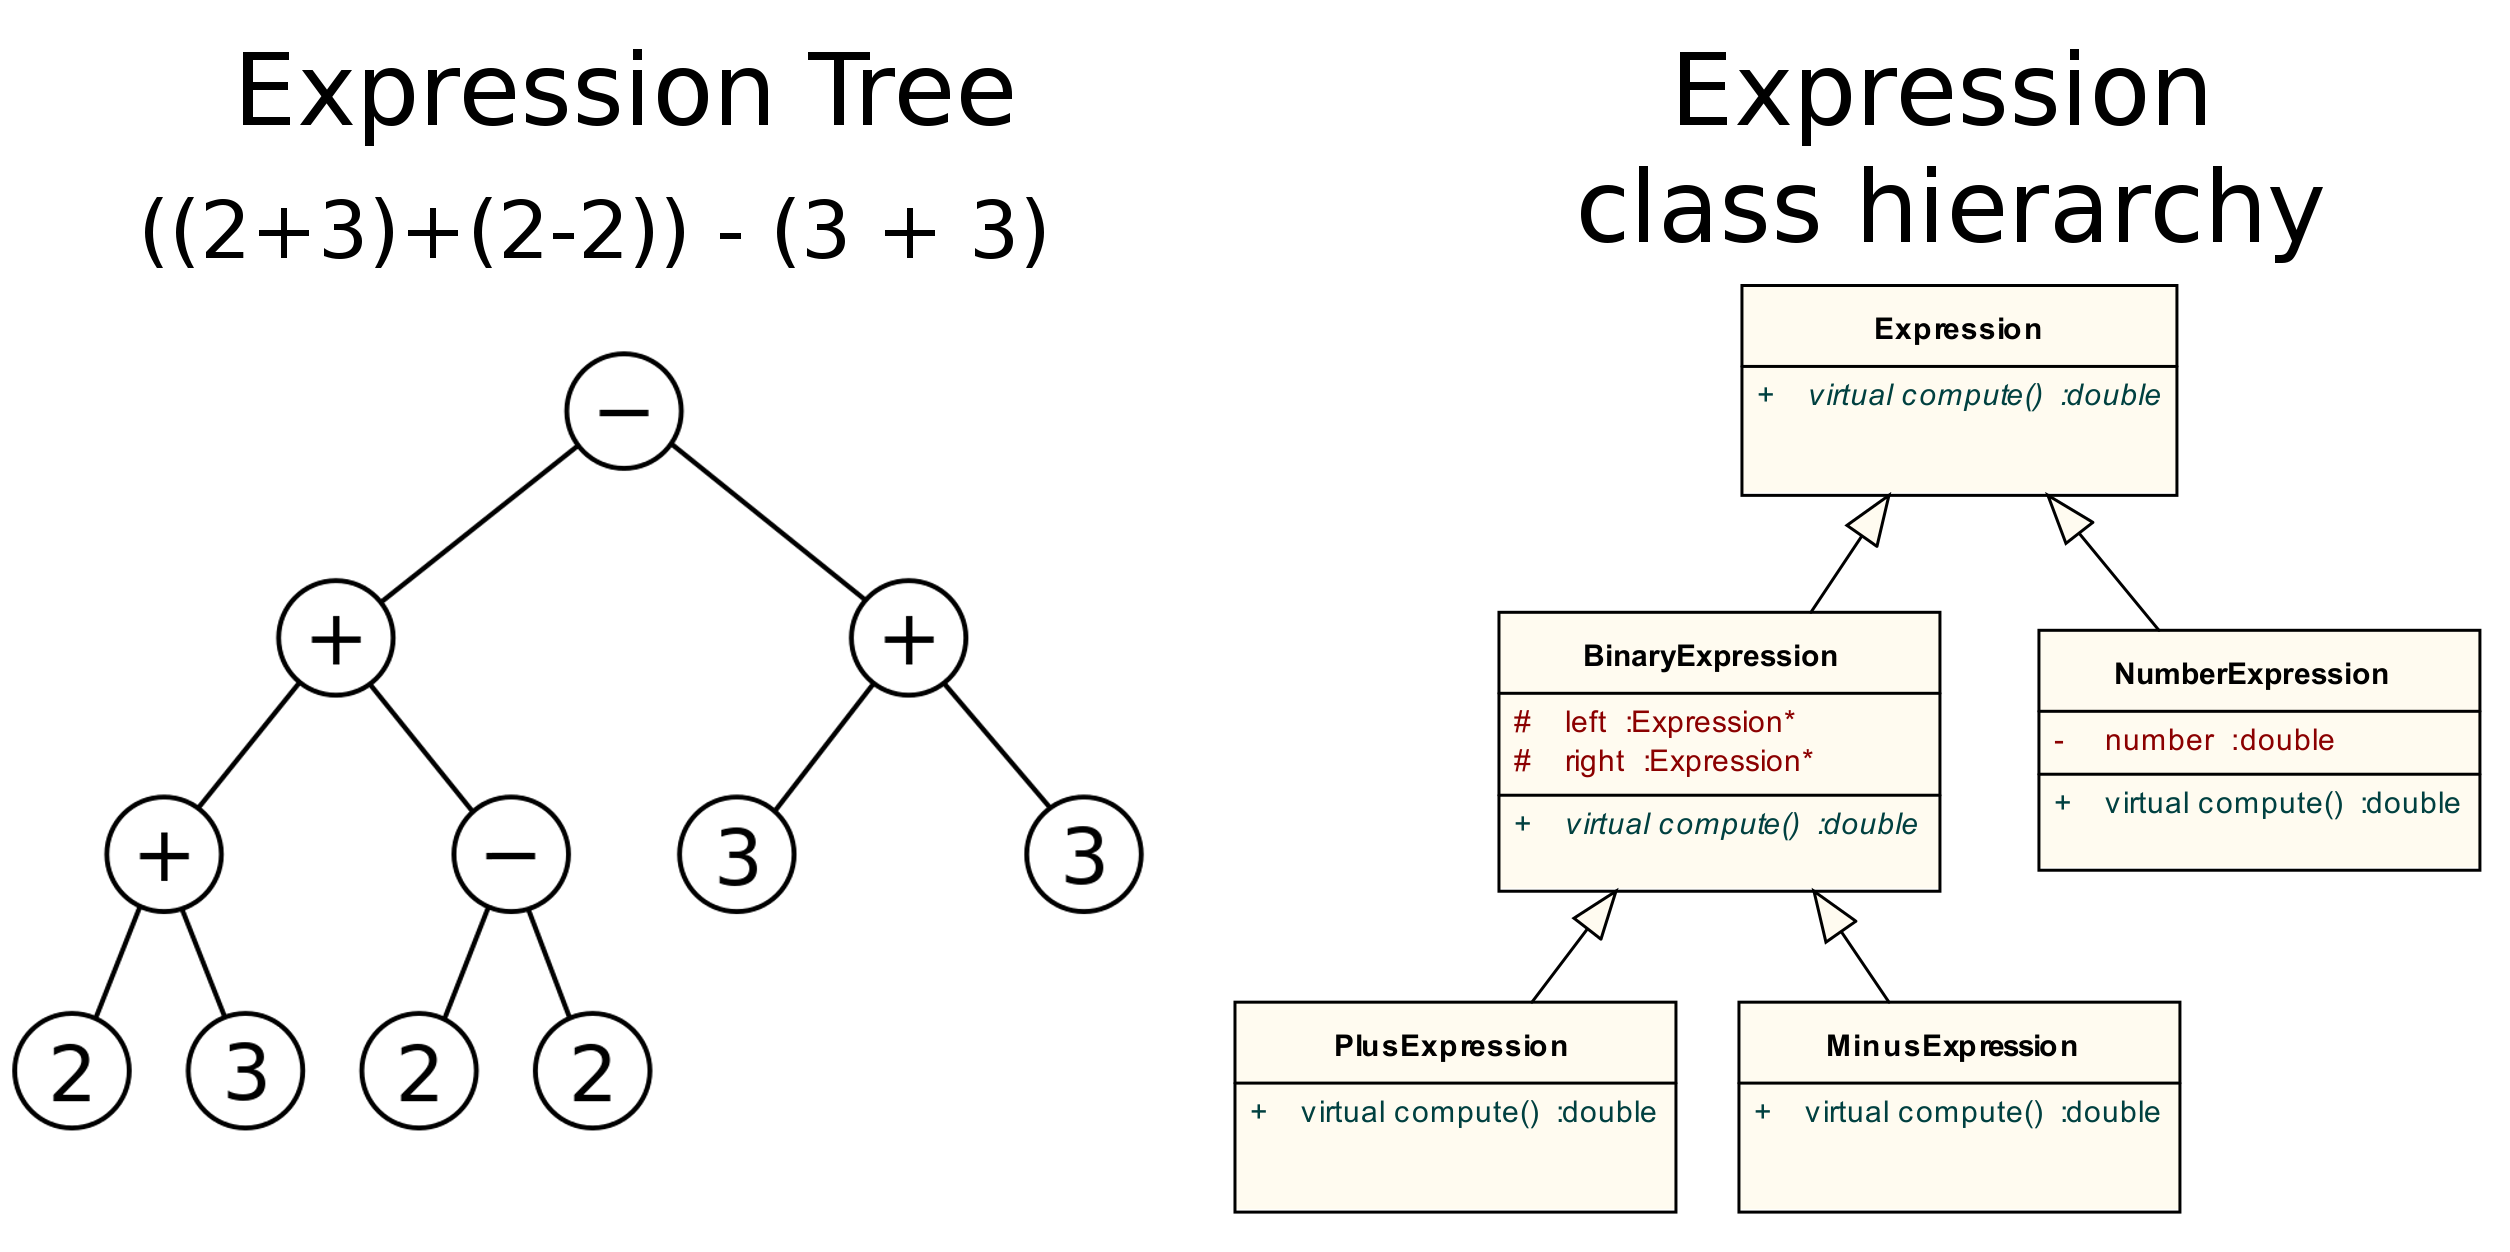
\includegraphics[width=1\textwidth]{ExpressionTree.png}

\begin{enumerate}

\item Schreiben Sie die abstrakte Klasse \emph{Expression}. Diese soll als Basisklasse für alle Ausdrücke dienen. Implementieren Sie einen parameterlosen Konstruktor und einen virtuellen Destruktor, die je eine Meldung auf der Konsole ausgeben, sodass es bei der Ausführung ersichtlich wird, wann eine \emph{Expression} erzeugt und wann zerstört wird. Deklarieren Sie außerdem eine abstrakte (pure virtual) Methode \textbf{double compute()}, die das Ergebnis des Ausdrucks berechnen und zurückgeben soll. 

\item Schreiben Sie die Klasse \emph{NumberExpression}, die ein Blatt mit einer Zahl darstellt. Dementsprechend soll \emph{NumberExpression} von \emph{Expression} erben und ein Attribut zum Speichern einer Zahl besitzen, der im Konstruktor initialisiert wird. Implementieren Sie den Konstruktor und virtuellen Destruktor und versehen Sie auch diese mit einer Konsolenausgabe. Implementieren Sie die Methode \emph{compute()}, die die gespeicherte Zahl zurückgibt.

\item Schreiben Sie die abstrakte Klasse \emph{BinaryExpression} mit den protected Attributen \emph{Expression* left, *right}. Implementieren Sie den Konstruktor und virtuellen Destruktor mit entsprechender Ausgabe. Vergessen Sie nicht, im Destruktor die beiden Zweige zu löschen. 

\item Schreiben Sie die Klassen \emph{PlusExpression} und \emph{MinusExpression}, die von \emph{BinaryExpression} erben und eine Addition bzw. Subtraktion realisieren. Implementieren Sie die Kon- und Destruktoren sowie die \emph{compute()} Methode.

\item Testen Sie Ihre Implementierung. Schauen Sie sich die Ausgabe genau an und versuchen Sie anhand der gegebenen Klassenhierarchie die Reihenfolge der Erzeugung und Zerstörung von Objekten  nachzuvollziehen.

\end{enumerate}

\section{Fortsetzung Aufzugsimulator}
Unser bisheriger Aufzugsimulator hat eine feste Strategie, nach der die einzelnen Stockwerke abgefahren werden. Mithilfe von Polymorphie können wir den Simulator so erweitern, dass die Strategie austauschbar wird.  

\begin{enumerate}
\item
Lagern Sie die bereits existierende Simulation des Aufzugs aus der \emph{main}-Funktion in eine eigene Funktion \emph{runSimulation()} aus. Die Funktion sollte das volle Gebäude als Parameter entgegennehmen und eine Liste (\emph{std::list<int>}) der angefahrenen Stockwerke zurückgeben. Überlegen Sie sich, auf welche Art das Gebäude idealerweise übergeben werden sollte. Testen Sie Ihre Implementierung.

\item Implementieren Sie die Klasse \emph{ElevatorStrategy}. Diese soll die Basisklasse für verschiedene Aufzugstrategien sein.

\begin{lstlisting}
/**
 * Elevator strategy base class. Used to determine at which floor the elevator should move next.
 */
class ElevatorStrategy {
public:
	virtual ~ElevatorStrategy();

	/**
	 * Creates a plan for the simulation. 
	 * Default implementation does nothing but saving the building pointer.
	 */
	virtual void createPlan(const Building*);

	/** 
	 * get next floor to visit.
	 */
	virtual int nextFloor() = 0;

protected:
	/** Pointer to current building, set by createPlan() */
	const Building* building;
};
\end{lstlisting}

Damit die Strategie das Gebäude nicht selbst modifizieren kann, wird \emph{Building} per const Pointer übergeben.

\item Implementieren Sie eine einfache Aufzugstrategie. Diese soll Folgendermaßen vorgehen: falls der Aufzug momentan leer ist, soll zum tiefsten Stockwerk gefahren werden, wo sich noch Personen befinden. Falls der Aufzug nicht leer ist, wird das Zielstockwerk eines der Personen im Aufzug ausgewählt.

\item Ändern Sie nun \emph{runSimulation()} entsprechend um, sodass die Simulation anhand der gegebenen Strategie durchführt wird. Folgender Pseudocode kann Ihnen als Denkhilfe dienen: \\
\begin{algorithm}[H]
 \SetAlgoLined
 \While{People in Building or Elevator}{
   Calculate next floor;\\
   
   Move Elevator to next floor; \\
   Let all arrived people off; \\
   Let all people on floor into Elevator;\\
 }
\end{algorithm}

\item Testen Sie Ihre Implementierung mit der bisher erstellten, einfachen Strategie.

\item Entwickeln Sie eigene Aufzugstrategien. Versuchen Sie, verschiedene Größen zu Optimieren, wie z.B. die Anzahl der Stopps oder die verbrauchte Energie. Hierfür können Sie Backtracking verwenden (siehe Wikipedia), eine einfache Methode, um optimale Lösungen durch Ausprobieren zu finden. Beachten Sie, dass der Aufzug auch kopiert werden kann, um verschiedene Strategien zu testen.

\end{enumerate}

\end{document}
